\section{Current state of the project}

\subsection[Debian]{Debian}
\nopagebreak[4]{
Debian continues its work toward ensuring that all of the packages in the distribution are bit-by-bit reproducible. 
To continuously check the status of reproducibility of individual packages, testing infrastructure is set up, reporting results on \autocite{tests-rbo}.
For the packages that are not reproducible for the tested variations, the diffoscope output is provided. That allows for an easier identification of underlying issues.\\
All the issues are inspected and categorized by people taking part in the Reproducible Builds project. Meaningful diffoscope output allows for a easier identification of issues at this step.\\
Figure \ref{fig:stats_issues} illustrates the process of identifying new issues that cause packages to be not reproducible. Figure \ref{fig:stats_notes} shows statistics about number of packages with notes attached to them, meaning that there is an identified issue or some sort of comment for them attached to them.\\
\begin{figure}
\centering
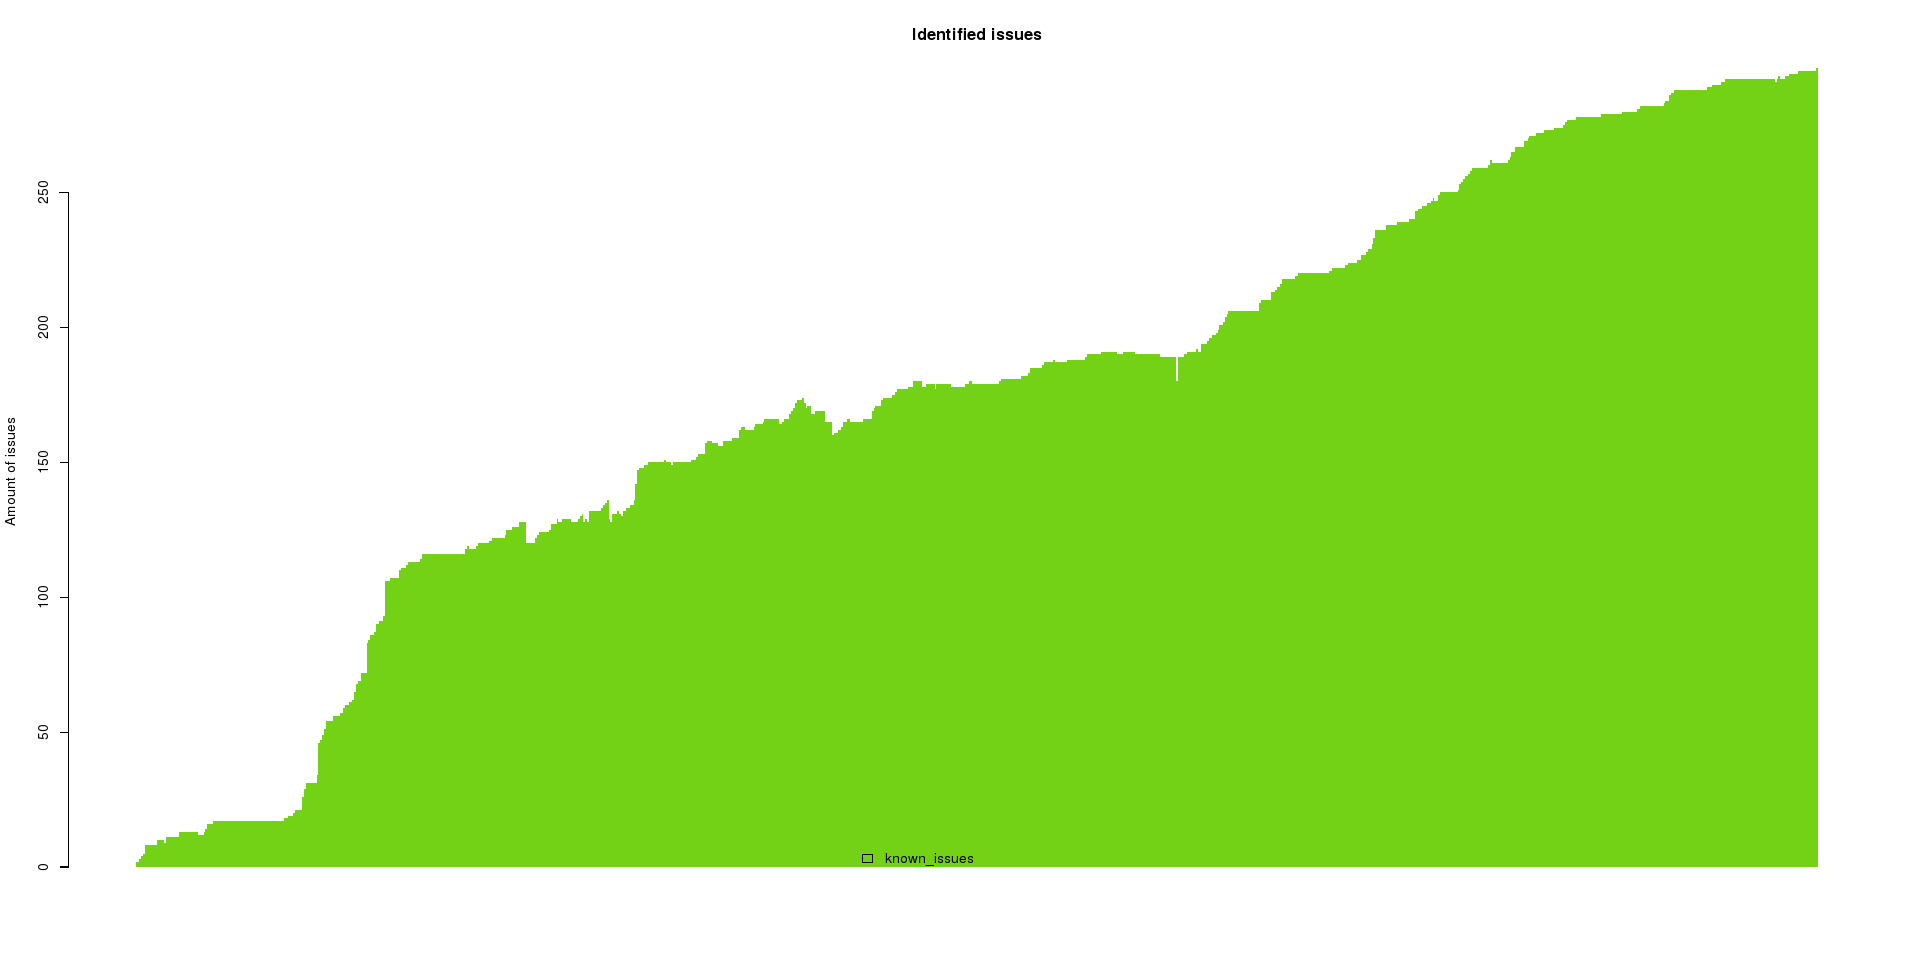
\includegraphics[width=0.95\textwidth]{fig/stats_issues.png}
\caption{\label{fig:stats_issues}Number of categorized reproducibility issues.}
\end{figure}
\begin{figure}
\centering
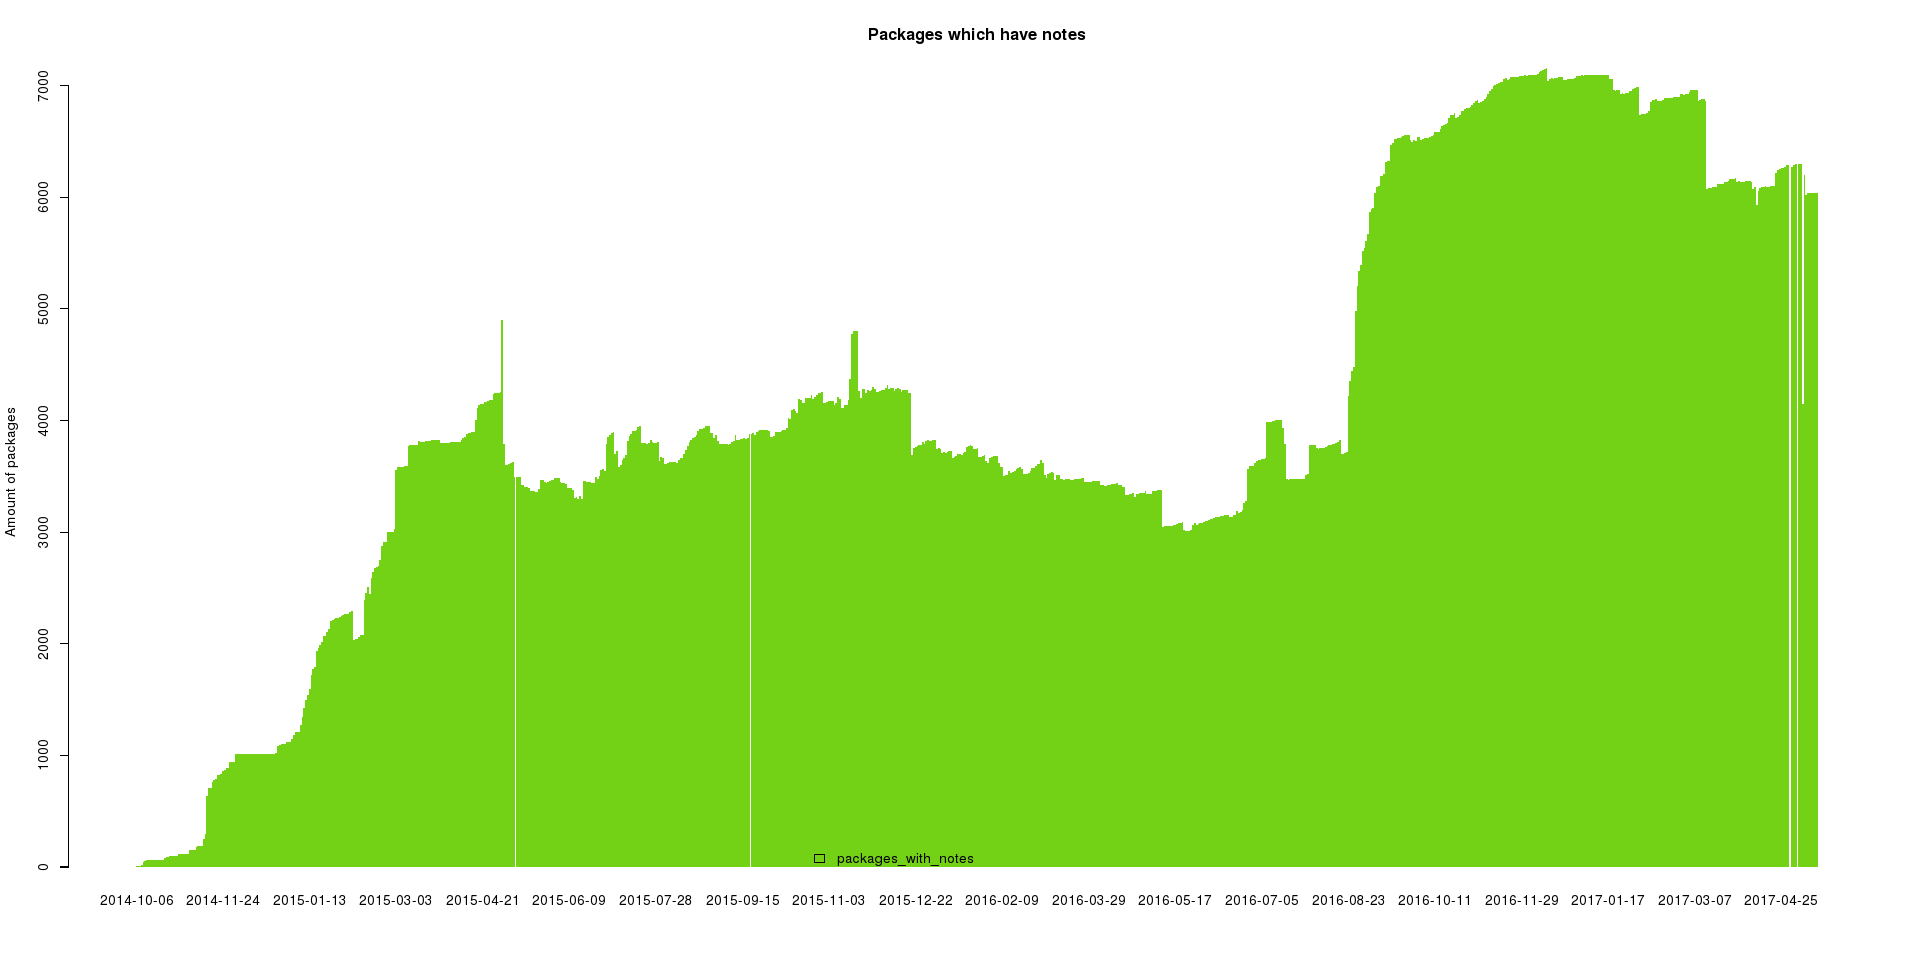
\includegraphics[width=0.95\textwidth]{fig/stats_notes.png}
\caption{\label{fig:stats_notes}Number of packages that have notes.}
\end{figure}
The nest step after the issue is identified is to fix it. For that, members of the project contact the maintainers of the packages with suggested edits. They collaborate with them to explain an issue and provide a ready way to fix it, so usually maintainers only have to accept the proposed patch.\\
Figure \ref{fig:stats_sid} shows the current status of reproducibility of Debian packages for unstable (sid) version of the distribution built for the amd64 target architecture.\\
\begin{figure}
\centering
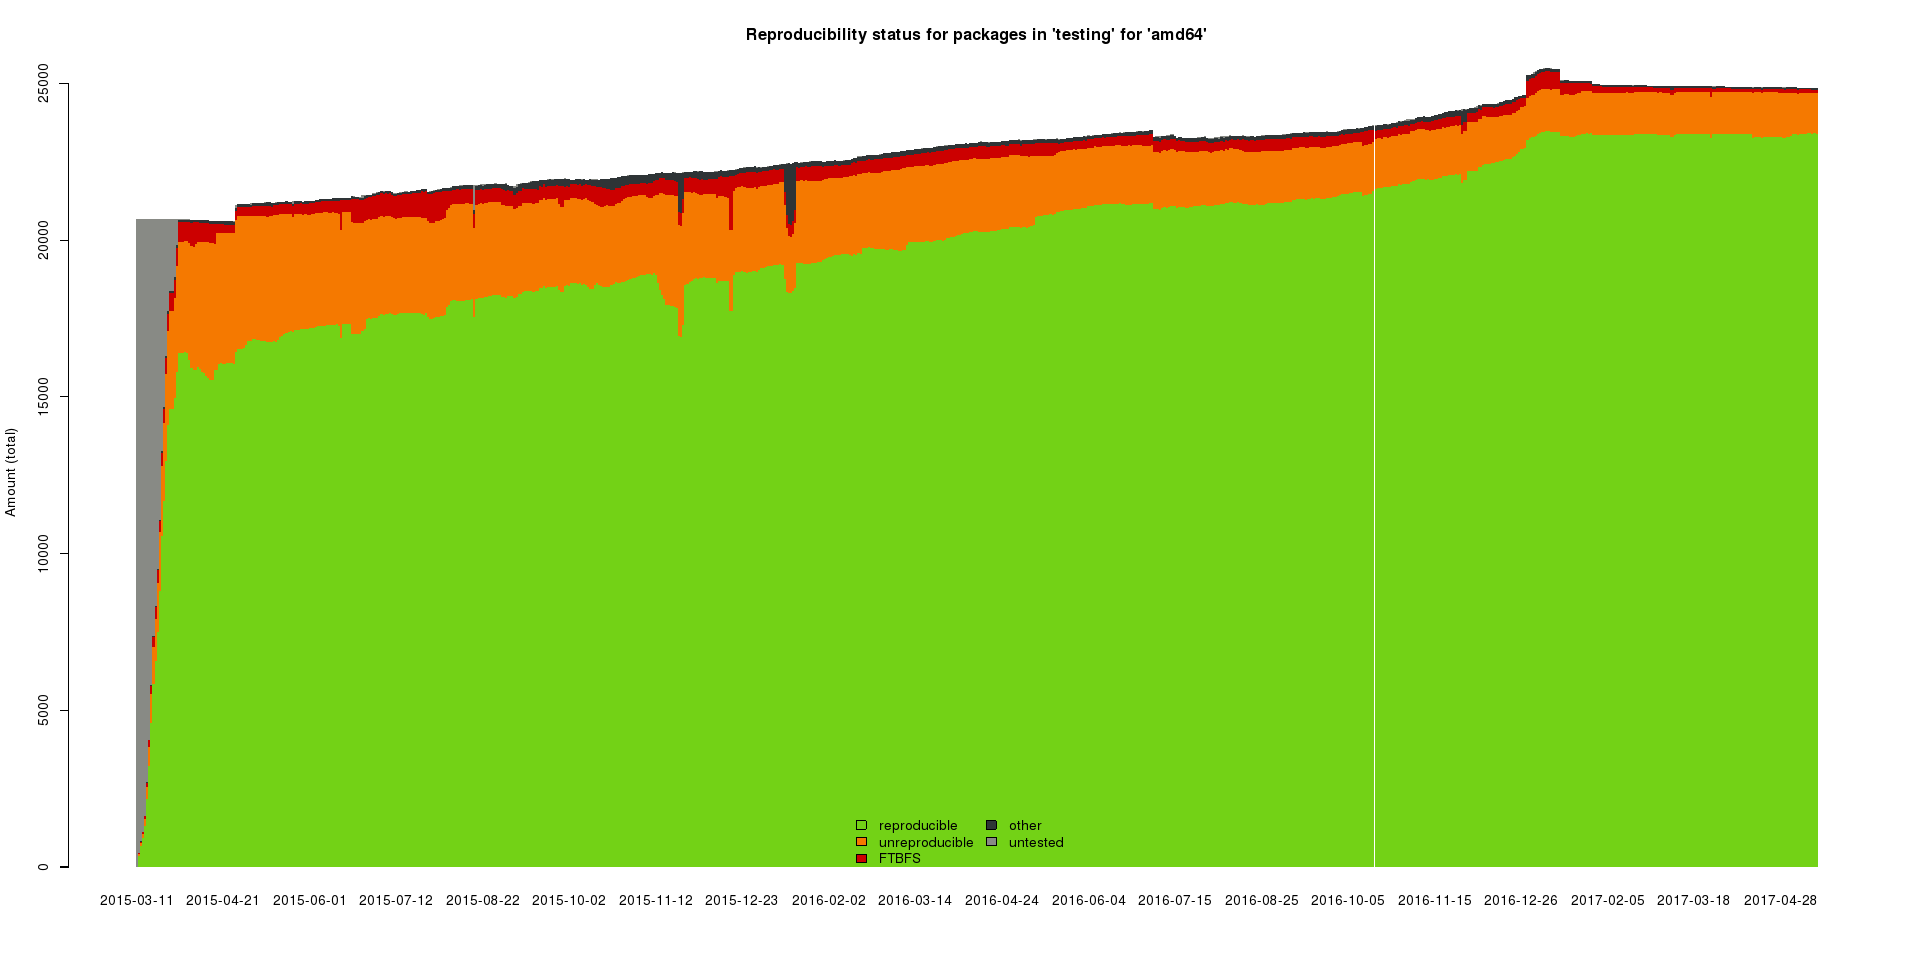
\includegraphics[width=0.95\textwidth]{fig/stats_pkg_state.png}
\caption{\label{fig:stats_sid}Overview of reproducible builds for packages in Debian unstable for amd64 architecture.}
\end{figure}

}
\subsection[F-droid]{F-droid}
\nopagebreak[4]{
The F-Droid project, that aims to provide an environment of free software for Android smartphones, has set up its own Verification Server. It functions in the similar fashion as Debian test infrastructure, rebuilding packages and providing the diffoscope output when results do not match.\\
}
\subsection[Other projects]{Other projects}
\nopagebreak[4]{
FreeBSD and NetBSD distributions also continue their work on reproducible builds. Currently, they use less variations between builds than Debian does, but within these constraint, they have achieved significant progress: NetBSD reported 100\% reproducibility within their build system in \autocite{netBSD} and FreeBSD is at 99.6\% at the moment \autocite{freeBSD}.
}


%\cleardoublepage
